\documentclass{article}
\usepackage[spanish]{babel}
\usepackage{graphicx}

\title{Cómputo Concurrente 2024-2 \\ Práctica 3 \\  Calabozos}

\author{Natalia Abigail Pérez Romero\\
Jonathan Bautista Parra \\ Valeria Reyes Tapia}

\date{\today}

\begin{document}

\maketitle
\section{Introduction}
En esta práctica se implementó un programa en Java que simula una variante del Problema de los Prisioneros.

\textbf{Problema de los Prisioneros:} Existen $N$ prisioneros y un guardia. El 
guardia. El guardia les comenta a los prisioneros: \textit{Pasare a un prisionero a la vez a un cuarto $D$, en este cuarto hay un interruptor $L$ (que tiene dos estados ON/OFF). Cada prisionero visitará el cuarto $D$ con frecuencia arbitraria. En cualquier momento un prisionero debe declarar "Ya hemos pasado todos". Si es correcto, todos los prisioneros serán liberados, de lo contrario serán aventados a los cocodrilos.}

Crea un algoritmo concurrente que ayude a los prisioneros a ser liberados, en este caso, supon que no conoces el estado inicial del interruptor $L$.

Toma en cuenta que:
\begin{itemize}
    \item Solo tenemos 1 interruptor.
    \item No se conoce el estado inicial del interruptor.
    \item Pasan de manera pseudoaleatoria a los prisioneros.
\end{itemize}

Se generará la simulación en el main.

\section{Solución Propuesta}
La clase Prisionero es la encargada de simular el comportamiento de un prisionero. El cual tiene los atributos:
\begin{itemize}
    \item \texttt{int id}: Identificador del prisionero.
    \item \texttt{boolean esVocero}: Indica si el prisionero es el vocero.
    \item \texttt{boolean marcado}: Indica si el prisionero ya ha pasado a la habitación.
    \item \texttt{int vecesPasadas}: Indica cuántas veces ha pasado el prisionero a la habitación.
\end{itemize}

La clase Vocero extiende de Prisionero y es la encargada de declarar si todos los prisioneros han pasado a la habitación. El vocero es el prisionero con el id 0. Tiene los mismo atributos que la clase Prisionero, y además tiene el atributo \texttt{Integer contador} que indica cuántos prisioneros han pasado a la habitación.

La clase Habitacion es la encargada de simular el comportamiento de la habitación, guarda el estado del interruptor (ON/OFF) y controla el acceso a la habitación.
Inicia con el interruptor en estado aleatorio.

Cuando un prisionero entra a la habitación, verifica que si el interruptor esta apagado, ha pasado menos de dos veces y no es vocero, entonces prende el interruptor, aumenta el contador de veces que ha pasado y se marca como que ya pasó.

Si el interruptor está prendido y el prisionero es el vocero, apaga el interruptor y aumenta el contador. Si el contado es mayor o igual a $(2*Prisioneros-1)$ entonces declara que todos han pasado.

La clase Main implenta la interfaz Runnable y es la encargada de crear los hilos de los prisioneros y crea la habitación.
Dentro del método run, mientras el Vocero no haya declarado que todos han pasado, pasa a un prisionero a la habitación (no tenemos control sobre que prisionero es).

\subsubsection*{De manera informal:}
La idea es que  cada prisionero que no sea el contador ponga el interruptor en ON 2 veces y que el que cuenta lo apague $2n$ veces así, de las 2 veces que el prisionero que no cuenta pone el interruptor en ON,  al menos 1 fue porque el que cuenta puso el interruptor en OFF. Y de las 2 veces que el prisionero que cuenta pone el interruptor en OFF,  al menos $n$ fue porque los $n$ prisioneros lo pusieron en ON

\section{Cuestionario}

Tu solución propuesta cumple:
\subsubsection*{Exclusión Mutua}

Sí, ya que se utiliza un candado dentro de la clase Main para controlar el acceso a la habitación. Un reentrantLock es un candado que permite que un hilo que ya tiene el candado lo vuelva a tomar sin que se bloquee. Y una vez que el hilo (que representa al prisionero) libera el candado, otro hilo puede tomarlo.

\subsubsection*{No Deadlock}
Sí. Para demostrarlo por contradicción supongamos que se da un deadlock. Esto implica que ningún prisionero puede entrar a la habitación. Pero esto no puede pasar, ya que el candado es reentrant, por lo que si un prisionero ya tiene el candado, puede volver a tomarlo sin que se bloquee. Por lo que no puede haber un deadlock. 

\subsubsection*{Libre de Hambruna}

Sí. Para demostrarlo por contradicción supongamos que se da un caso de hambruna. Esto implica que un prisionero nunca entra a la habitación, esto pasaría si el candado no le permite entrar lo que implica que otro prisionero siempre lo toma. Pero esto no puede pasar, ya que los prisioneros siempre salen de la habitación, por lo que el candado siempre se libera. Por lo que no puede haber un caso de hambruna.

\begin{itemize}
    \item ¿Tu solución cumple para $n$ prisioneros?
    
    Sí. El vocero se encarga de declarar que todos han pasado a la habitación, contando cuántas veces apago el interruptor ($2n-1$). Y los prisioneros se encargan de prender el interruptor y marcar que ya pasaron.

    \item Si tu programa tarda mucho en terminar, ¿por qué crees que pasa esto?
    
    Tarda en ejecutar cuando la cantidad de prisioneros es muy grande, ya que el vocero tiene que esperar a que todos los prisioneros pasen a la habitación dos veces.

    \item De la pregunta anterior, que podrias proponer para mejorar los tiempos.
    
    Podría mejorar los tiempos si el vocero no tuviera que esperar a que todos los prisioneros pasen dos veces a la habitación, pero sin saber el estado inicial del interruptor, no se me ocurre una manera de hacerlo.
    
\end{itemize}

\subsection{Analiza el siguiente enunciado:}
\texttt{"Si los candados cumplen con exclusión mutua, no deadlock o libre de hambruna, es decir, con las propiedades para un candado seguro, entonces el sistema donde lo utilizaremos también las cumplirá."} De esto justifica porque si se cumple o no.

El enunciado no se cumple, dado que el sistema puede tener otros problemas que no estén relacionados con el candado, como por ejemplo, un mal diseño del sistema, un mal manejo de los recursos, entre otros.

\subsection{Diagrama UML}
\begin{center}
        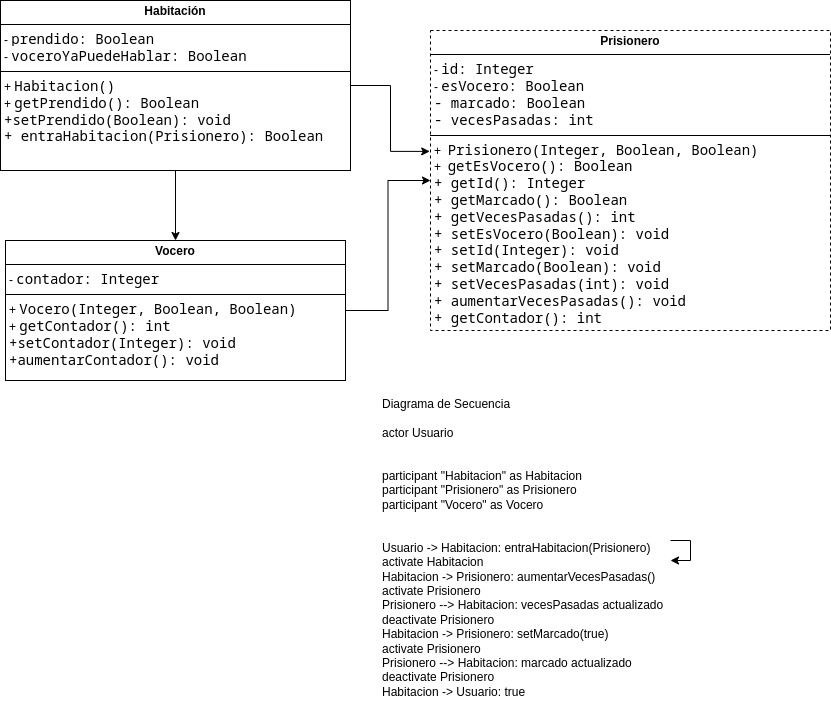
\includegraphics[width=1\linewidth]{Practica3.drawio.png}
\end{center}

\end{document}
